\PassOptionsToPackage{unicode=true}{hyperref} % options for packages loaded elsewhere
\PassOptionsToPackage{hyphens}{url}
%
\documentclass[11pt,ignorenonframetext,]{beamer}
\setbeamertemplate{caption}[numbered]
\setbeamertemplate{caption label separator}{: }
\setbeamercolor{caption name}{fg=normal text.fg}
\beamertemplatenavigationsymbolsempty
\usepackage{lmodern}
\usepackage{amssymb,amsmath}
\usepackage{ifxetex,ifluatex}
\usepackage{fixltx2e} % provides \textsubscript
\ifnum 0\ifxetex 1\fi\ifluatex 1\fi=0 % if pdftex
  \usepackage[T1]{fontenc}
  \usepackage[utf8]{inputenc}
  \usepackage{textcomp} % provides euro and other symbols
\else % if luatex or xelatex
  \usepackage{unicode-math}
  \defaultfontfeatures{Ligatures=TeX,Scale=MatchLowercase}
\fi
\usetheme[]{metropolis}
% use upquote if available, for straight quotes in verbatim environments
\IfFileExists{upquote.sty}{\usepackage{upquote}}{}
% use microtype if available
\IfFileExists{microtype.sty}{%
\usepackage[]{microtype}
\UseMicrotypeSet[protrusion]{basicmath} % disable protrusion for tt fonts
}{}
\IfFileExists{parskip.sty}{%
\usepackage{parskip}
}{% else
\setlength{\parindent}{0pt}
\setlength{\parskip}{6pt plus 2pt minus 1pt}
}
\usepackage{hyperref}
\hypersetup{
            pdftitle={Lecture 14},
            pdfborder={0 0 0},
            breaklinks=true}
\urlstyle{same}  % don't use monospace font for urls
\newif\ifbibliography
\usepackage{color}
\usepackage{fancyvrb}
\newcommand{\VerbBar}{|}
\newcommand{\VERB}{\Verb[commandchars=\\\{\}]}
\DefineVerbatimEnvironment{Highlighting}{Verbatim}{commandchars=\\\{\}}
% Add ',fontsize=\small' for more characters per line
\newenvironment{Shaded}{}{}
\newcommand{\AlertTok}[1]{\textcolor[rgb]{1.00,0.00,0.00}{\textbf{#1}}}
\newcommand{\AnnotationTok}[1]{\textcolor[rgb]{0.38,0.63,0.69}{\textbf{\textit{#1}}}}
\newcommand{\AttributeTok}[1]{\textcolor[rgb]{0.49,0.56,0.16}{#1}}
\newcommand{\BaseNTok}[1]{\textcolor[rgb]{0.25,0.63,0.44}{#1}}
\newcommand{\BuiltInTok}[1]{#1}
\newcommand{\CharTok}[1]{\textcolor[rgb]{0.25,0.44,0.63}{#1}}
\newcommand{\CommentTok}[1]{\textcolor[rgb]{0.38,0.63,0.69}{\textit{#1}}}
\newcommand{\CommentVarTok}[1]{\textcolor[rgb]{0.38,0.63,0.69}{\textbf{\textit{#1}}}}
\newcommand{\ConstantTok}[1]{\textcolor[rgb]{0.53,0.00,0.00}{#1}}
\newcommand{\ControlFlowTok}[1]{\textcolor[rgb]{0.00,0.44,0.13}{\textbf{#1}}}
\newcommand{\DataTypeTok}[1]{\textcolor[rgb]{0.56,0.13,0.00}{#1}}
\newcommand{\DecValTok}[1]{\textcolor[rgb]{0.25,0.63,0.44}{#1}}
\newcommand{\DocumentationTok}[1]{\textcolor[rgb]{0.73,0.13,0.13}{\textit{#1}}}
\newcommand{\ErrorTok}[1]{\textcolor[rgb]{1.00,0.00,0.00}{\textbf{#1}}}
\newcommand{\ExtensionTok}[1]{#1}
\newcommand{\FloatTok}[1]{\textcolor[rgb]{0.25,0.63,0.44}{#1}}
\newcommand{\FunctionTok}[1]{\textcolor[rgb]{0.02,0.16,0.49}{#1}}
\newcommand{\ImportTok}[1]{#1}
\newcommand{\InformationTok}[1]{\textcolor[rgb]{0.38,0.63,0.69}{\textbf{\textit{#1}}}}
\newcommand{\KeywordTok}[1]{\textcolor[rgb]{0.00,0.44,0.13}{\textbf{#1}}}
\newcommand{\NormalTok}[1]{#1}
\newcommand{\OperatorTok}[1]{\textcolor[rgb]{0.40,0.40,0.40}{#1}}
\newcommand{\OtherTok}[1]{\textcolor[rgb]{0.00,0.44,0.13}{#1}}
\newcommand{\PreprocessorTok}[1]{\textcolor[rgb]{0.74,0.48,0.00}{#1}}
\newcommand{\RegionMarkerTok}[1]{#1}
\newcommand{\SpecialCharTok}[1]{\textcolor[rgb]{0.25,0.44,0.63}{#1}}
\newcommand{\SpecialStringTok}[1]{\textcolor[rgb]{0.73,0.40,0.53}{#1}}
\newcommand{\StringTok}[1]{\textcolor[rgb]{0.25,0.44,0.63}{#1}}
\newcommand{\VariableTok}[1]{\textcolor[rgb]{0.10,0.09,0.49}{#1}}
\newcommand{\VerbatimStringTok}[1]{\textcolor[rgb]{0.25,0.44,0.63}{#1}}
\newcommand{\WarningTok}[1]{\textcolor[rgb]{0.38,0.63,0.69}{\textbf{\textit{#1}}}}
\usepackage{longtable,booktabs}
\usepackage{caption}
% These lines are needed to make table captions work with longtable:
\makeatletter
\def\fnum@table{\tablename~\thetable}
\makeatother
% Prevent slide breaks in the middle of a paragraph:
\widowpenalties 1 10000
\raggedbottom
\setbeamertemplate{part page}{
\centering
\begin{beamercolorbox}[sep=16pt,center]{part title}
  \usebeamerfont{part title}\insertpart\par
\end{beamercolorbox}
}
\setbeamertemplate{section page}{
\centering
\begin{beamercolorbox}[sep=12pt,center]{part title}
  \usebeamerfont{section title}\insertsection\par
\end{beamercolorbox}
}
\setbeamertemplate{subsection page}{
\centering
\begin{beamercolorbox}[sep=8pt,center]{part title}
  \usebeamerfont{subsection title}\insertsubsection\par
\end{beamercolorbox}
}
\AtBeginPart{
  \frame{\partpage}
}
\AtBeginSection{
  \ifbibliography
  \else
    \frame{\sectionpage}
  \fi
}
\AtBeginSubsection{
  \frame{\subsectionpage}
}
\setlength{\emergencystretch}{3em}  % prevent overfull lines
\providecommand{\tightlist}{%
  \setlength{\itemsep}{0pt}\setlength{\parskip}{0pt}}
\setcounter{secnumdepth}{0}

% set default figure placement to htbp
\makeatletter
\def\fps@figure{htbp}
\makeatother

\usepackage{geometry}
\usepackage{graphicx}

\usepackage{bbold}
\usepackage{lmodern}


\usepackage{url}		% produces hyperlinks

\usepackage{colortbl}	% allows for color usage in tables
\usepackage{multirow}	% allows for rows that span multiple rows in tables

\usepackage{color}          	% gives color options
\usepackage{xcolor}		% this package has a variety of color options

\usepackage{multicol}
\usepackage{textcomp}

\usepackage{setspace}
\usepackage{changepage}
\usepackage{isotope}

\singlespacing

%%%%%%%%%%%%%%%%
% Small code output
%%%%%%%%%%%%%%%%

%% change fontsize of R code

\makeatletter
\@ifundefined{Shaded}{\newenvironment{Shaded}{}{}}{}
\makeatother


\let\oldShaded\Shaded
\let\endoldShaded\endShaded
\renewenvironment{Shaded}{\footnotesize\begin{spacing}{0.9}\oldShaded}{\endoldShaded\end{spacing}}

%% change fontsize of output
\let\oldverbatim\verbatim
\let\endoldverbatim\endverbatim
\renewenvironment{verbatim}{\footnotesize\begin{spacing}{0.9}\oldverbatim}{\endoldverbatim\end{spacing}}


\newcommand{\tinyoutput}{
  \renewenvironment{Shaded}{\tiny\begin{spacing}{0.9}\oldShaded}{\endoldShaded\end{spacing}}
  \renewenvironment{verbatim}{\tiny\begin{spacing}{0.9}\oldverbatim}{\endoldverbatim\end{spacing}}
}

\newcommand{\scriptoutput}{
  \renewenvironment{Shaded}{\scriptsize\begin{spacing}{0.9}\oldShaded}{\endoldShaded\end{spacing}}
  \renewenvironment{verbatim}{\scriptsize\begin{spacing}{0.9}\oldverbatim}{\endoldverbatim\end{spacing}}
}

\newcommand{\footnoteoutput}{
  \renewenvironment{Shaded}{\footnotesize\begin{spacing}{0.9}\oldShaded}{\endoldShaded\end{spacing}}
  \renewenvironment{verbatim}{\footnotesize\begin{spacing}{0.9}\oldverbatim}{\endoldverbatim\end{spacing}}
}

%\newcommand{\verbatimfont}[1]{\renewcommand{\verbatim@font}{\ttfamily#1}}


%%%%%%%%%%%%%%%%
% Custom Colors
%%%%%%%%%%%%%%%%

\definecolor{redhl}{rgb}{0.98,0.29,0.28}
\definecolor{yellowhl}{rgb}{0.98,0.87,0.28}


\xdefinecolor{oiBlue}{rgb}{0.15, 0.35, 0.55}
\xdefinecolor{gray}{rgb}{0.5, 0.5, 0.5}
\xdefinecolor{darkGray}{rgb}{0.3, 0.3, 0.3}
\xdefinecolor{darkerGray}{rgb}{0.2, 0.2, 0.2}
\xdefinecolor{rubineRed}{rgb}{0.89,0,0.30}
\xdefinecolor{linkCol}{rgb}{0.11,0.49,0.95}	
\xdefinecolor{irishGreen}{rgb}{0,0.60,0}	
\xdefinecolor{darkturquoise}{rgb}{0.44, 0.58, 0.86}
\definecolor{lightGreen}{rgb}{0.533,0.765,0.42}
%\xdefinecolor{hlblue}{rgb}{0.051,0.65,1}
\xdefinecolor{hlblue}{rgb}{ 0.055, 0.639, 0.831}
\definecolor{light}{rgb}{.337,.608,.741}
\definecolor{dark}{rgb}{.337,.608,.741}

\definecolor{cpink}{rgb}{0.93, 0.23, 0.51}

%%%%%%%%%%%%%%%%
% Custom Commands
%%%%%%%%%%%%%%%%

% text colors
\newcommand{\red}[1]{\textit{\textcolor{rubineRed}{#1}}}
\newcommand{\orange}[1]{\textit{\textcolor{orange}{#1}}}
\newcommand{\pink}[1]{\textit{\textcolor{rubineRed!90!white!50}{#1}}}
\newcommand{\green}[1]{\textit{\textcolor{irishGreen}{#1}}}
\newcommand{\blue}[1]{\textit{\textcolor{darkturquoise}{#1}}}
\newcommand{\light}[1]{\textcolor{light}{\textbf{#1}}}
\newcommand{\dark}[1]{\textcolor{dark}{#1}}
\newcommand{\gray}[1]{\textcolor{gray}{#1}}


% mail
\newcommand{\mail}[1]{\href{mailto:#1}{\textit{\textcolor{linkCol}{#1}}}}

% highlighting: hl, hlGr, mathhl
\newcommand{\hl}[1]{\textit{\textcolor{hlblue}{#1}}}
\newcommand{\hlGr}[1]{\textit{\textcolor{lightGreen}{#1}}}
\newcommand{\hlRd}[1]{\textit{\textcolor{rubineRed}{#1}}}
\newcommand{\mathhl}[1]{\textcolor{hlblue}{\ensuremath{#1}}}
\newcommand{\hlr}[1]{\fcolorbox{redhl}{white}{$\displaystyle #1$}}
\newcommand{\hly}[1]{\fcolorbox{yellowhl}{white}{$\displaystyle #1$}}


\newcommand{\vvfill}{\vskip0pt plus 1filll}

\DeclareMathOperator*{\argmin}{arg\,min}
\DeclareMathOperator*{\argmax}{arg\,max}

\title{Lecture 14}
\providecommand{\subtitle}[1]{}
\subtitle{Covariance Functions}
\date{3/08/2018}

\begin{document}
\frame{\titlepage}

\hypertarget{more-on-covariance-functions}{%
\section{More on Covariance
Functions}\label{more-on-covariance-functions}}

\begin{frame}[t]{%
\protect\hypertarget{nugget-covariance}{%
Nugget Covariance}}

\vspace{-5mm}

\[ Cov(y_{t_i}, y_{t_j}) = \sigma^2 {1}_{\{h=0\}} \text{   where } h = |t_i - t_j|\]

\vspace{5mm}

\begin{center}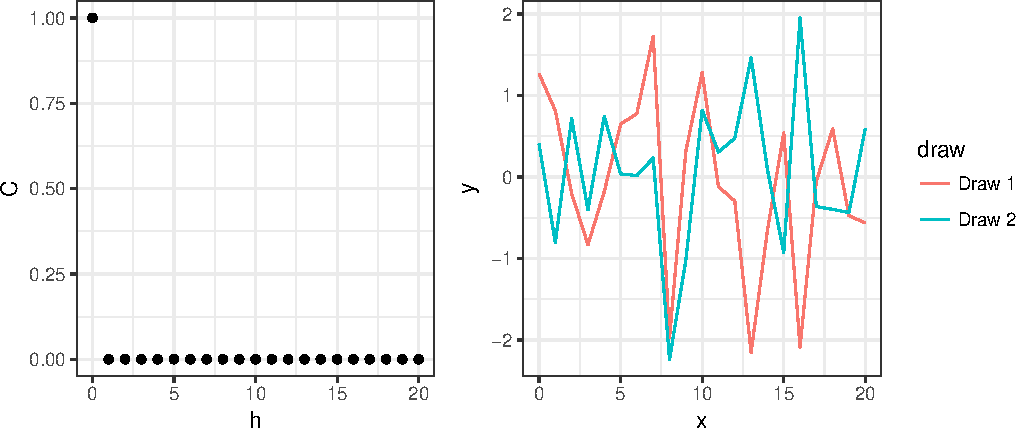
\includegraphics[width=\textwidth]{Lec14_files/figure-beamer/unnamed-chunk-1-1} \end{center}

\end{frame}

\begin{frame}[t]{%
\protect\hypertarget{power-square-exponential-covariance}{%
(- / Power / Square) Exponential Covariance}}

\vspace{-5mm}

\[ Cov(y_{t_i}, y_{t_j}) = \sigma^2\exp\left(-(h\,l)^p\right) \text{   where } h = |t_i - t_j|\]

\begin{center}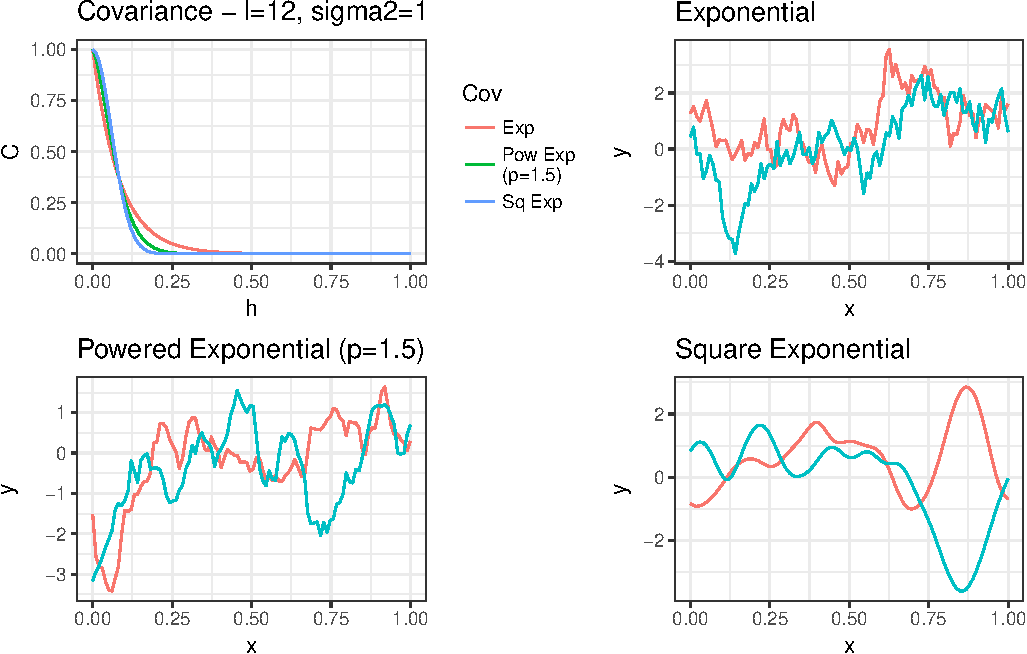
\includegraphics[width=\textwidth]{Lec14_files/figure-beamer/unnamed-chunk-2-1} \end{center}

\end{frame}

\begin{frame}[t]{%
\protect\hypertarget{matern-covariance}{%
Matern Covariance}}

\vspace{-10mm}

\[ Cov(y_{t_i}, y_{t_j}) = \sigma^2 ~ \frac{2^{1-\nu}}{\Gamma(\nu)} ~ \left(\sqrt{2\nu}\, h \cdot l\right)^\nu ~ K_\nu\left(\sqrt{2\nu} \, h \cdot l\right) \text{   where } h = |t_i - t_j|\]

\begin{center}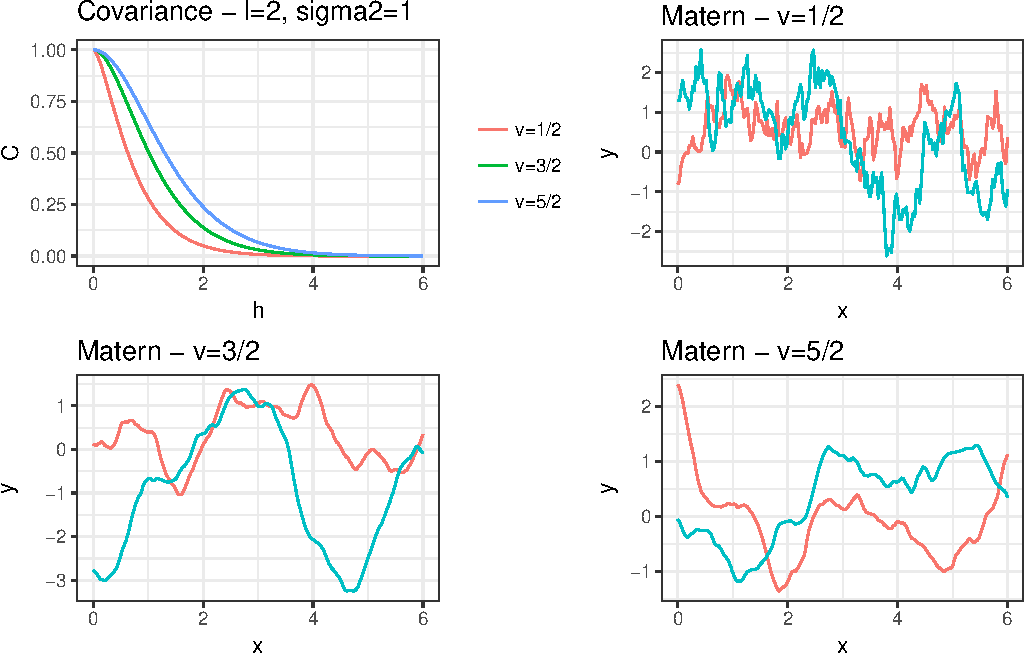
\includegraphics[width=\textwidth]{Lec14_files/figure-beamer/unnamed-chunk-3-1} \end{center}

\end{frame}

\begin{frame}[t]{%
\protect\hypertarget{matern-covariance-1}{%
Matern Covariance}}

\begin{itemize}
\tightlist
\item
  \(K_\nu\) is the modified Bessel function of the second kind.
\end{itemize}

\vspace{1mm}

\begin{itemize}
\tightlist
\item
  A Gaussian process with Matérn covariance has sample functions that
  are \(\lceil \nu -1\rceil\) times differentiable.
\end{itemize}

\vspace{1mm}

\begin{itemize}
\tightlist
\item
  When \(\nu = 1/2 + p\) for \(p \in \mathbb{N}^+\) then the Matern has
  a simplified form (product of an exponential and a polynomial of order
  \(p\)).
\end{itemize}

\vspace{1mm}

\begin{itemize}
\tightlist
\item
  When \(\nu = 1/2\) the Matern is equivalent to the exponential
  covariance.
\end{itemize}

\vspace{1mm}

\begin{itemize}
\tightlist
\item
  As \(\nu \to \infty\) the Matern converges to the square exponential
  covariance.
\end{itemize}

\vspace{1mm}

\begin{itemize}
\tightlist
\item
  A Gaussian process with Matérn covariance has paths that are
  \(\lceil \nu \rceil -1\) times differentiable.
\end{itemize}

\end{frame}

\begin{frame}[t]{%
\protect\hypertarget{rational-quadratic-covariance}{%
Rational Quadratic Covariance}}

\vspace{-5mm}

\[ Cov(y_{t_i}, y_{t_j}) = \sigma^2 \left(1 + \frac{h^2 \, l^2}{\alpha}\right)^{-\alpha} \text{   where } h = |t_i - t_j|\]

\begin{center}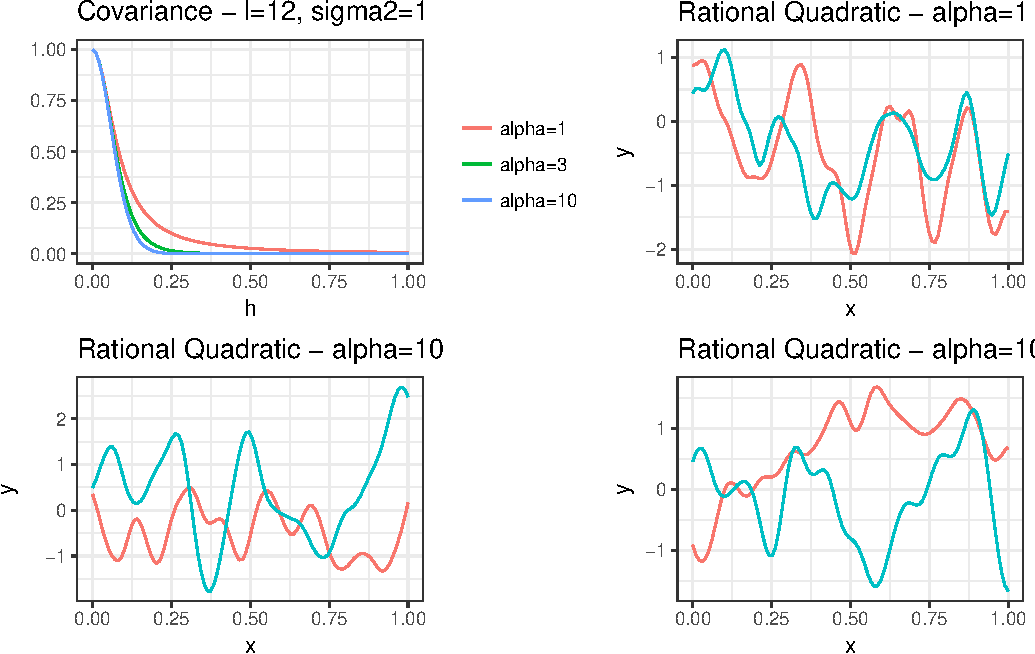
\includegraphics[width=\textwidth]{Lec14_files/figure-beamer/unnamed-chunk-4-1} \end{center}

\end{frame}

\begin{frame}[t]{%
\protect\hypertarget{rational-quadratic-covariance-1}{%
Rational Quadratic Covariance}}

\begin{itemize}
\tightlist
\item
  is a scaled mixture of squared exponential covariance functions with
  different characteristic length-scales (\(l\)).
\end{itemize}

\vspace{1mm}

\begin{itemize}
\tightlist
\item
  As \(\alpha \to \infty\) the rational quadratic converges to the
  square exponential covariance.
\end{itemize}

\vspace{1mm}

\begin{itemize}
\tightlist
\item
  Has sample functions that are infinitely differentiable for any value
  of \(\alpha\)
\end{itemize}

\end{frame}

\begin{frame}[t]{%
\protect\hypertarget{spherical-covariance}{%
Spherical Covariance}}

\vspace{-10mm}
\footnotesize

\[ Cov(y_{t_i}, y_{t_j}) = \begin{cases}
\sigma^2\left(1 - \frac{3}{2} h \cdot l + \frac{1}{2} (h \cdot l)^3)\right) & \text{if   } 0 < h < 1/l \\
0 & \text{otherwise}
\end{cases} \text{   where } h = |t_i - t_j|\]

\begin{center}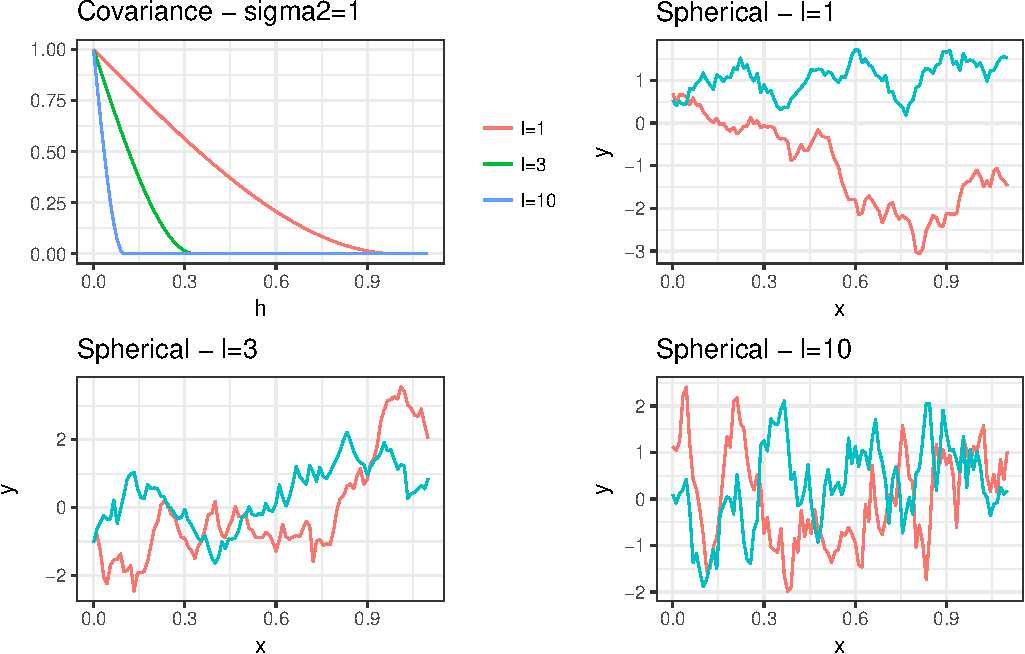
\includegraphics[width=\textwidth]{Lec14_files/figure-beamer/unnamed-chunk-5-1} \end{center}

\end{frame}

\begin{frame}[t]{%
\protect\hypertarget{periodic-covariance}{%
Periodic Covariance}}

\vspace{-10mm}

\[ Cov(y_{t_i}, y_{t_j}) = \sigma^2 \exp\left(-2\, l^2 \sin^2\left(\pi\frac{h}{p}\right)\right)  \text{   where } h = |t_i - t_j| \]

\begin{center}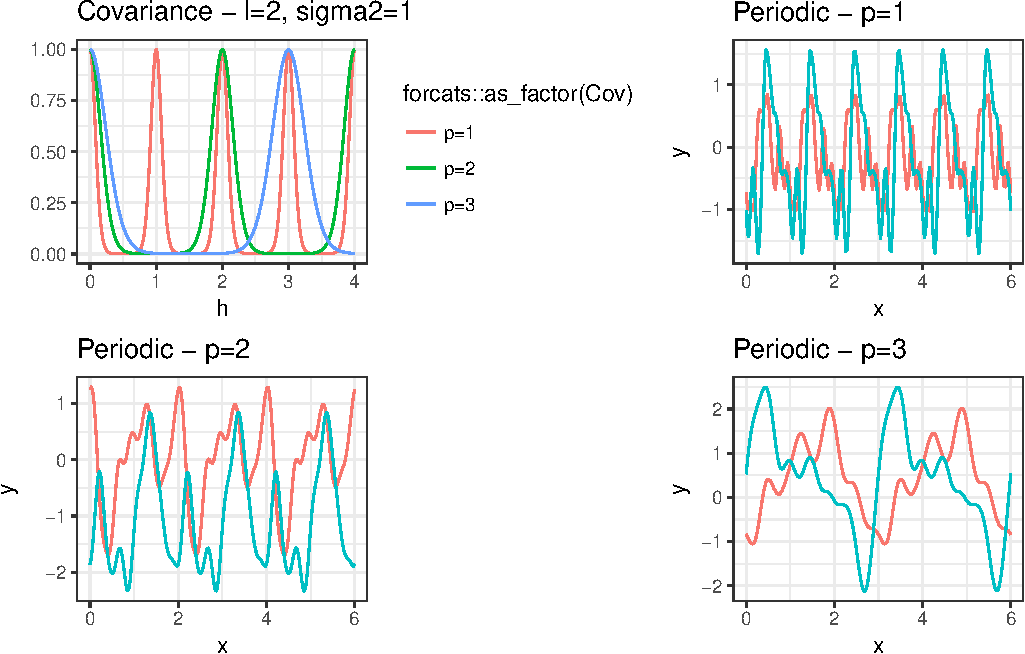
\includegraphics[width=\textwidth]{Lec14_files/figure-beamer/unnamed-chunk-6-1} \end{center}

\end{frame}

\begin{frame}[t]{%
\protect\hypertarget{linear-covariance}{%
Linear Covariance}}

\vspace{-5mm}

\[ Cov(y_{t_i}, y_{t_j}) = \sigma^2_b + \sigma^2_v~(t_i-c)(t_j-c)\]

\begin{center}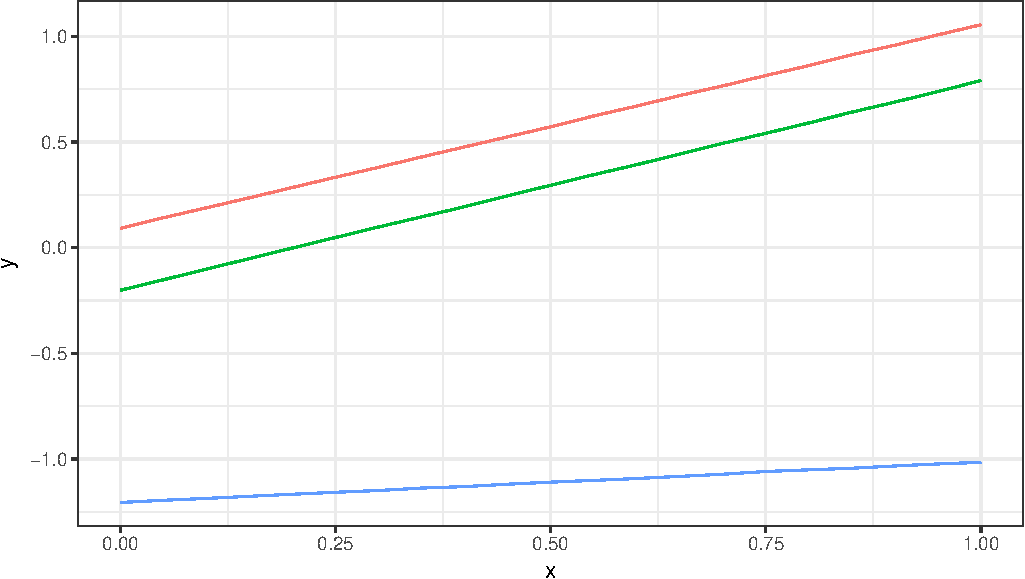
\includegraphics[width=0.7\textwidth]{Lec14_files/figure-beamer/unnamed-chunk-7-1} \end{center}

\end{frame}

\begin{frame}[t]{%
\protect\hypertarget{combining-covariances}{%
Combining Covariances}}

If we definite two valid covariance functions,
\(Cov_a(y_{t_i}, y_{t_j})\) and \(Cov_b(y_{t_i}, y_{t_j})\) then the
following are also valid covariance functions,

\[
\begin{aligned}
Cov_a(y_{t_i}, y_{t_j}) + Cov_b(y_{t_i}, y_{t_j}) \\
Cov_a(y_{t_i}, y_{t_j}) \times Cov_b(y_{t_i}, y_{t_j})
\end{aligned}
\]

\end{frame}

\begin{frame}[t]{%
\protect\hypertarget{linear-times-linear-to-quadratic}{%
Linear \(\times\) Linear \(\to\) Quadratic}}

\vspace{-5mm}

\[ Cov_a(y_{t_i}, y_{t_j}) = 1 + 2~(t_i \times t_j) \]
\[ Cov_b(y_{t_i}, y_{t_j}) = 2 + 1~(t_i \times t_j) \]

\begin{center}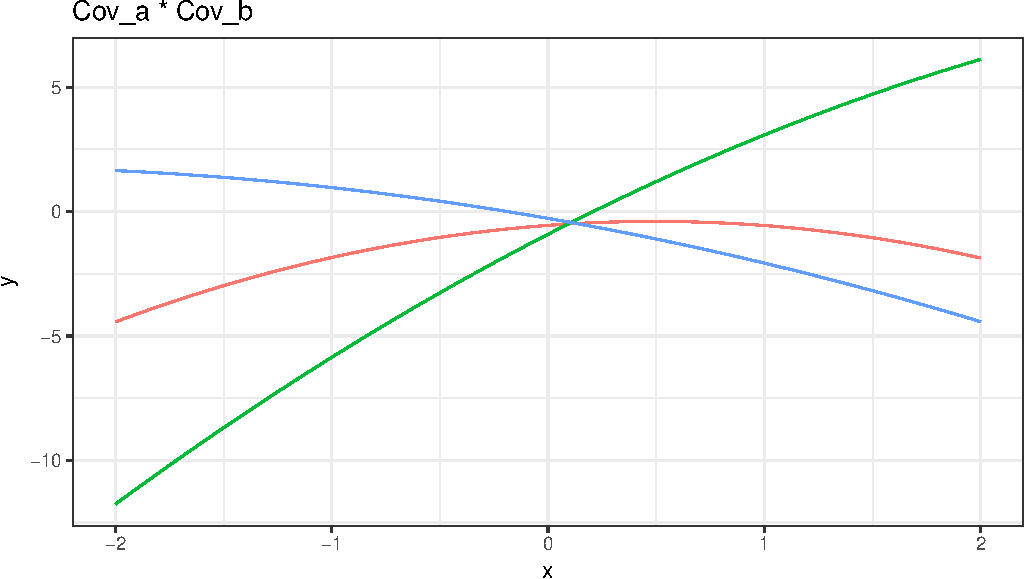
\includegraphics[width=\textwidth]{Lec14_files/figure-beamer/unnamed-chunk-8-1} \end{center}

\end{frame}

\begin{frame}[t]{%
\protect\hypertarget{linear-times-periodic}{%
Linear \(\times\) Periodic}}

\vspace{-5mm}

\[ Cov_a(y_{t_i}, y_{t_j}) = 1 + 1~(t_i \times t_j) \]
\[ Cov_b(y_{t_i}, y_{t_j}) = \exp\left(-2\, \sin^2\left(2\pi\,h\right)\right) \]

\begin{center}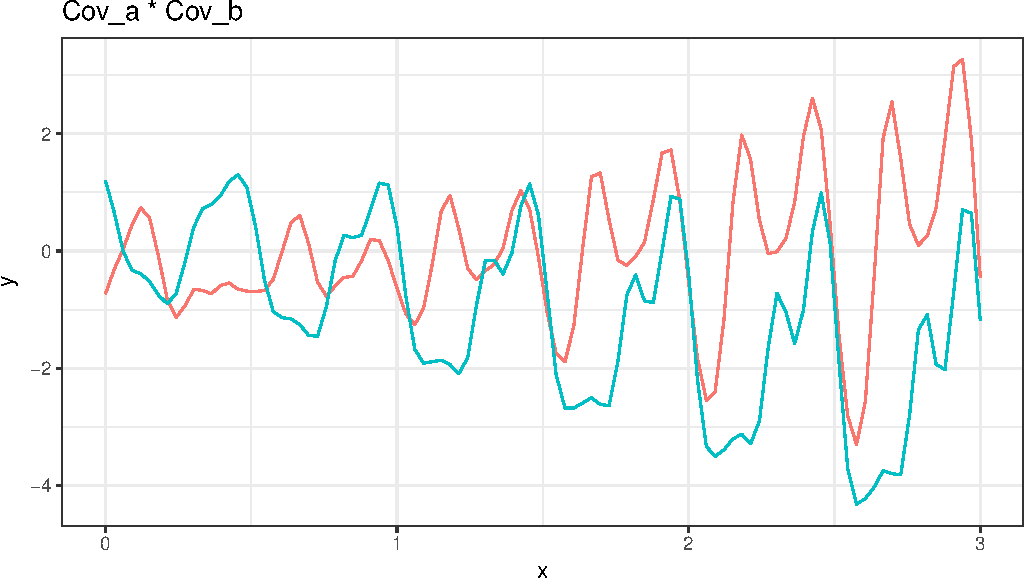
\includegraphics[width=\textwidth]{Lec14_files/figure-beamer/unnamed-chunk-9-1} \end{center}

\end{frame}

\begin{frame}[t]{%
\protect\hypertarget{linear-periodic}{%
Linear + Periodic}}

\vspace{-5mm}

\[ Cov_a(y_{t_i}, y_{t_j}) = 1 + 1~(t_i \times t_j) \]
\[ Cov_b(h = |t_i - t_j|) = \exp\left(-2\, \sin^2\left(2\pi\,h\right)\right) \]

\begin{center}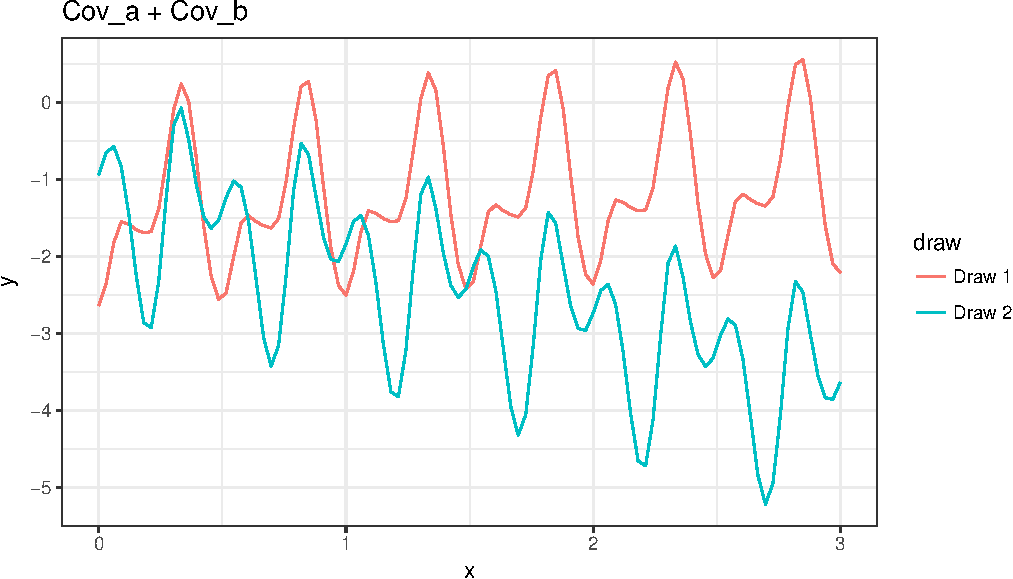
\includegraphics[width=\textwidth]{Lec14_files/figure-beamer/unnamed-chunk-10-1} \end{center}

\end{frame}

\begin{frame}[t]{%
\protect\hypertarget{sq-exp-times-periodic-to-locally-periodic}{%
Sq Exp \(\times\) Periodic \(\to\) Locally Periodic}}

\vspace{-5mm}

\[ Cov_a(h = |t_i - t_j|) =\exp(-(1/3)h^2) \]
\[ Cov_b(h = |t_i - t_j|) = \exp\left(-2\, \sin^2\left(\pi\,h\right)\right) \]

\begin{center}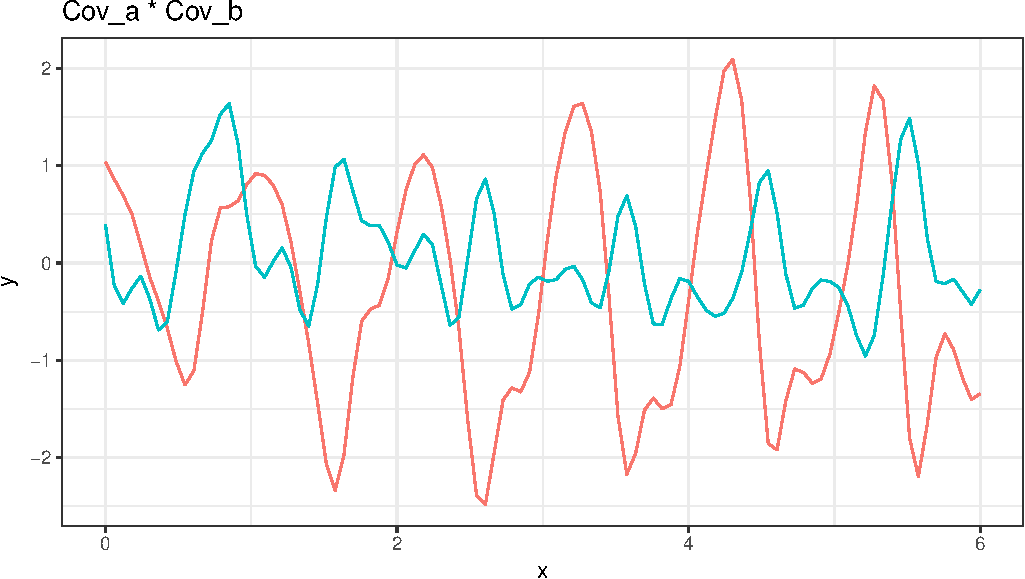
\includegraphics[width=\textwidth]{Lec14_files/figure-beamer/unnamed-chunk-11-1} \end{center}

\end{frame}

\begin{frame}[t]{%
\protect\hypertarget{sq-exp-short-sq-exp-long}{%
Sq Exp (short) + Sq Exp (long)}}

\vspace{-5mm}

\[ Cov_a(h = |t_i - t_j|) = (1/4) \exp(-4\sqrt{3}h^2) \]
\[ Cov_b(h = |t_i - t_j|) = \exp(-(\sqrt{3}/2)h^2) \]

\begin{center}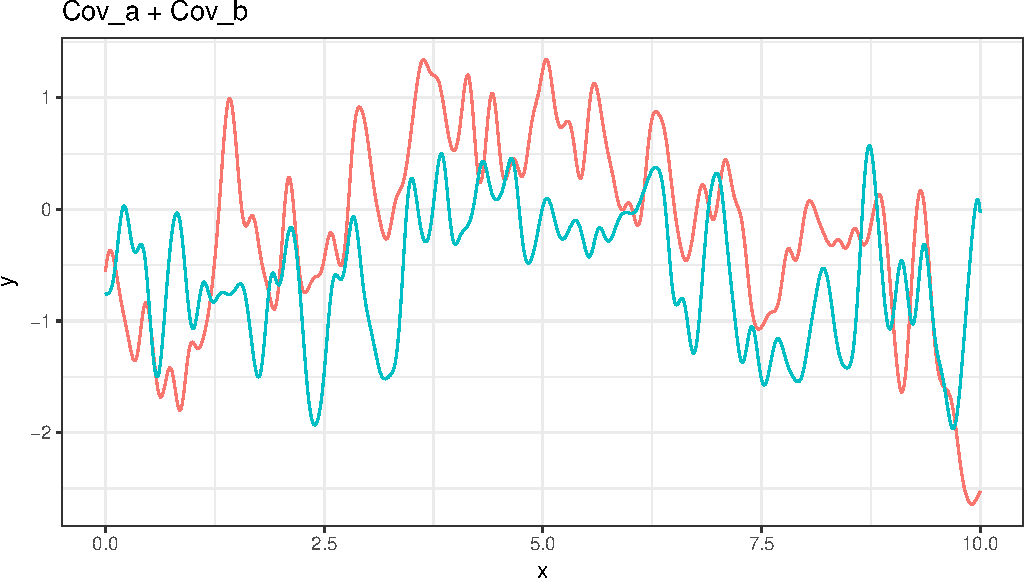
\includegraphics[width=\textwidth]{Lec14_files/figure-beamer/unnamed-chunk-12-1} \end{center}

\end{frame}

\begin{frame}[t]{%
\protect\hypertarget{sq-exp-short-sq-exp-long-seen-another-way}{%
Sq Exp (short) + Sq Exp (long) (Seen another way)}}

\begin{center}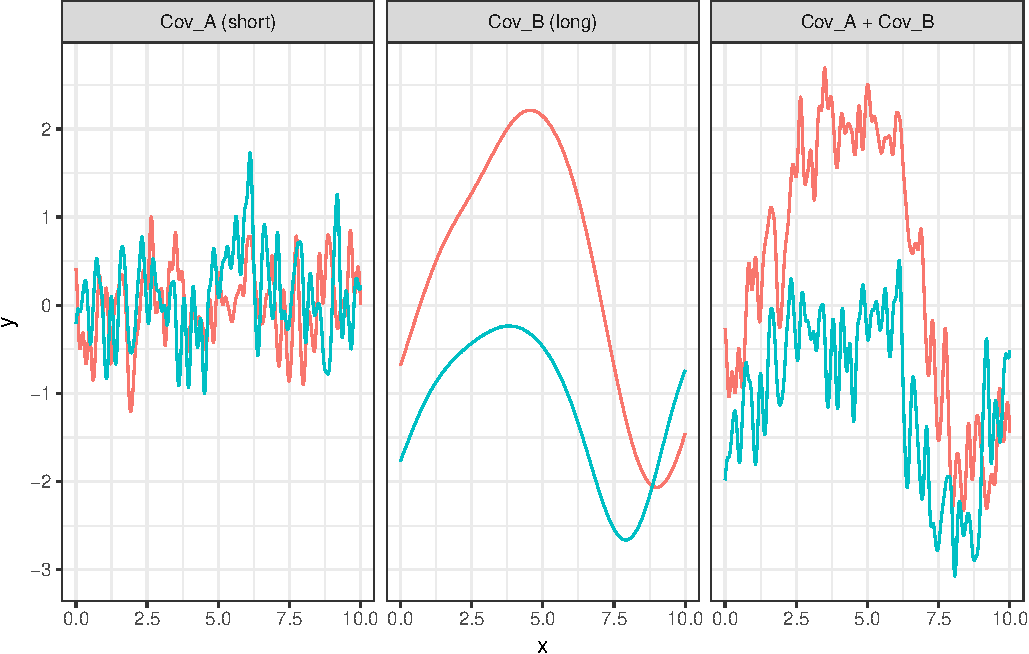
\includegraphics[width=\textwidth]{Lec14_files/figure-beamer/unnamed-chunk-13-1} \end{center}

\end{frame}

\hypertarget{bda3-example}{%
\section{BDA3 example}\label{bda3-example}}

\begin{frame}{%
\protect\hypertarget{bda3}{%
BDA3}}

\begin{center}
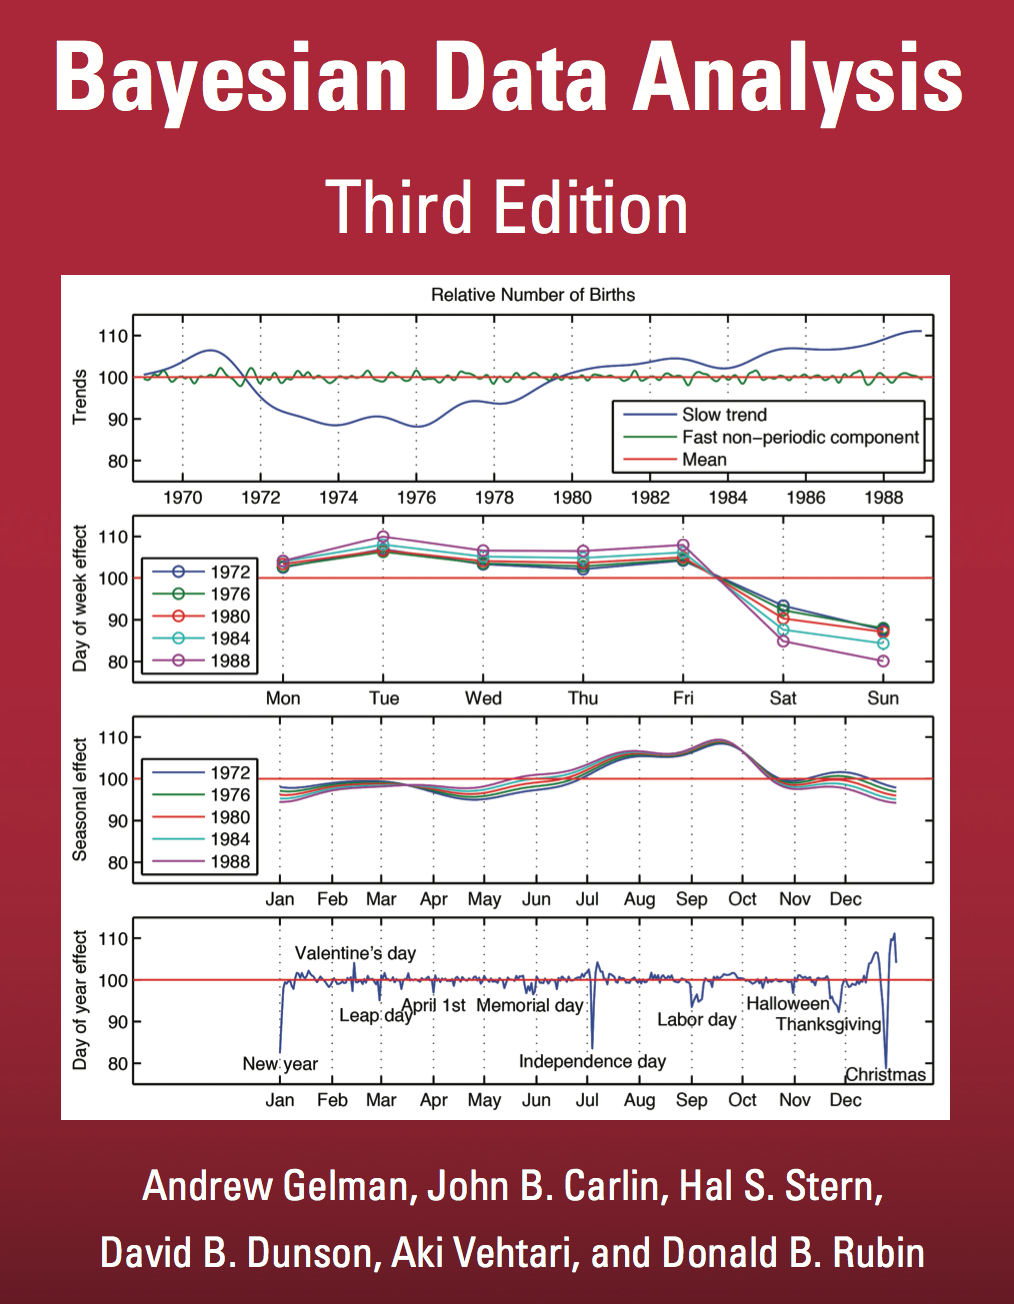
\includegraphics[width=0.7\textwidth]{figs/bda_cover.png} 

$~$

\vspace{-3mm}
\url{http://research.cs.aalto.fi/pml/software/gpstuff/demo_births.shtml}
\end{center}

\end{frame}

\begin{frame}{%
\protect\hypertarget{births-one-year}{%
Births (one year)}}

\begin{columns}
\begin{column}{0.5\textwidth}
\begin{center}
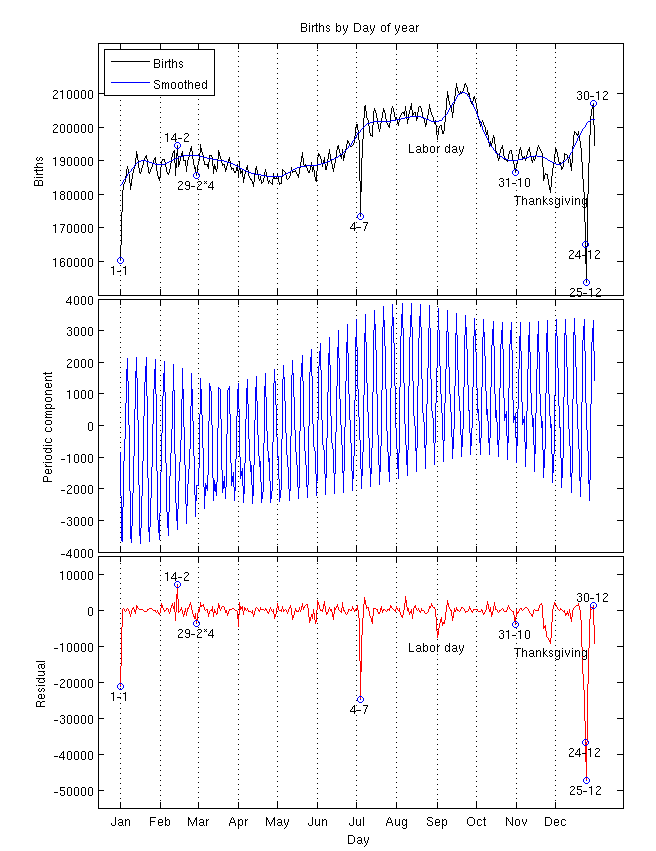
\includegraphics[width=\textwidth]{figs/births_pic1.png}
\end{center}
\end{column}
\begin{column}{0.5\textwidth}

1. Smooth long term trend \\ (\textit{sq exp cov})

\vspace{2mm}

2. Seven day periodic trend with decay (\textit{periodic $\times$ sq exp cov})

\vspace{2mm}

3. Constant mean

\end{column}
\end{columns}

\end{frame}

\begin{frame}[t]{%
\protect\hypertarget{component-contributions}{%
Component Contributions}}

We can view our GP in the following ways,

\[ \symbf{y} \sim \mathcal{N}(\symbf{\mu},~ \symbf{\Sigma}_1 + \symbf{\Sigma}_2 + \sigma^2 \symbf{I}\,) \]

but with appropriate conditioning we can also think of \(\symbf{y}\) as
being the sum of multipe independent GPs

\[ \symbf{y} = \symbf{\mu} + w_1(\symbf{t}) + w_2(\symbf{t}) + w_3(\symbf{t})\]
where \[
\begin{aligned}
w_1(\symbf{t}) &\sim \mathcal{N}(0, \symbf{\Sigma}_1) \\
w_2(\symbf{t}) &\sim \mathcal{N}(0, \symbf{\Sigma}_2) \\
w_3(\symbf{t}) &\sim \mathcal{N}(0, \sigma^2 \symbf{I}\,)
\end{aligned}
\]

\end{frame}

\begin{frame}[t]{%
\protect\hypertarget{decomposition-of-covariance-components}{%
Decomposition of Covariance Components}}

\footnotesize

\[ \begin{bmatrix} 
y \\
w_1 \\
w_2
\end{bmatrix} 
\sim \mathcal{N} \left(
\begin{bmatrix}
\symbf{\mu} \\ 0 \\ 0
\end{bmatrix},~
\begin{bmatrix}
\Sigma_1 + \Sigma_2 + \sigma^2 \symbf{I} & \Sigma_1 & \Sigma_2 \\
\Sigma_1 & \Sigma_1 & 0\\
\Sigma_2 & 0  & \Sigma_2 \\
\end{bmatrix}
\right)
\]

\normalsize

therefore

\[ w_1 ~|~ \symbf{y},\symbf{\mu},\symbf{\theta} \sim \mathcal{N}(\symbf{\mu}_{cond},~ \symbf{\Sigma}_{cond}) \]

\[ \symbf{\mu}_{cond} = 0 + \Sigma_1 ~ (\Sigma_1 + \Sigma_2 + \sigma^2 I)^{-1}(\symbf{y}-\symbf{\mu}) \]
\[ \symbf{\Sigma}_{cond} = \Sigma_1 - \Sigma_1 (\Sigma_1 + \Sigma_2 + \sigma^2 \symbf{I})^{-1} {\Sigma_1}^t \]

\end{frame}

\begin{frame}{%
\protect\hypertarget{births-multiple-years}{%
Births (multiple years)}}

\begin{adjustwidth}{-10mm}{-10mm}
\begin{center}
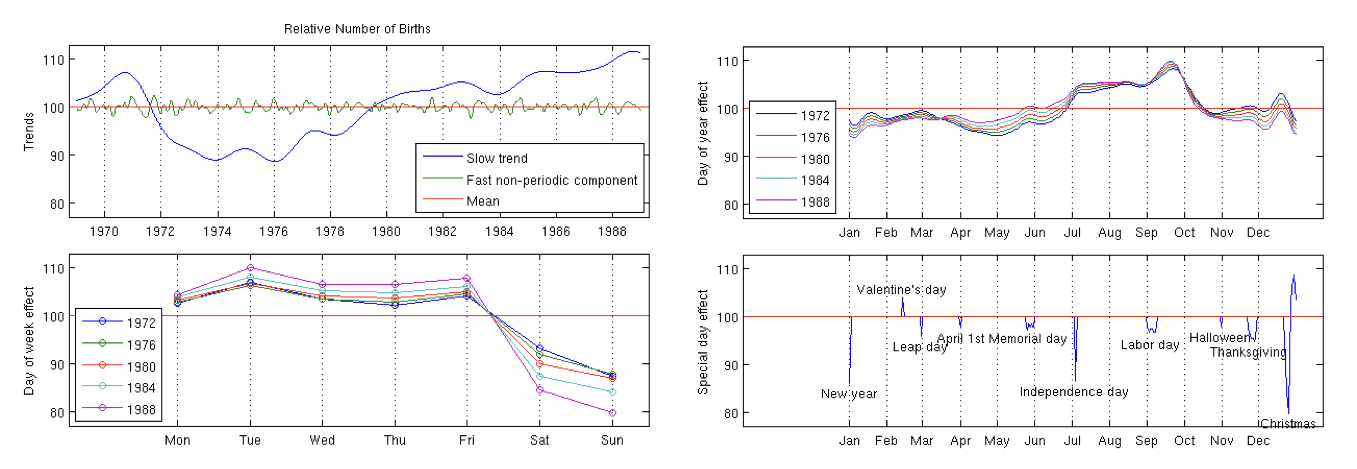
\includegraphics[width=\paperwidth]{figs/births_pic2.png}
\end{center}
\end{adjustwidth}

\vspace{-3mm}

\footnotesize

\begin{enumerate}
[1.]
\item
  slowly changing trend (\emph{sq exp cov})
\item
  small time scale correlating noise (\emph{sq exp cov})
\item
  7 day periodical component capturing day of week effect
  (\emph{periodic \(\times\) sq exp cov})
\item
  365.25 day periodical component capturing day of year effect
  (\emph{periodic \(\times\) sq exp cov})
\item
  component to take into account the special days and interaction with
  weekends (\emph{linear cov})
\item
  independent Gaussian noise (\emph{nugget cov})
\item
  constant mean
\end{enumerate}

\end{frame}

\hypertarget{mauna-loa-exampel}{%
\section{Mauna Loa Exampel}\label{mauna-loa-exampel}}

\begin{frame}{%
\protect\hypertarget{atmospheric-co_2}{%
Atmospheric CO\(_2\)}}

\begin{center}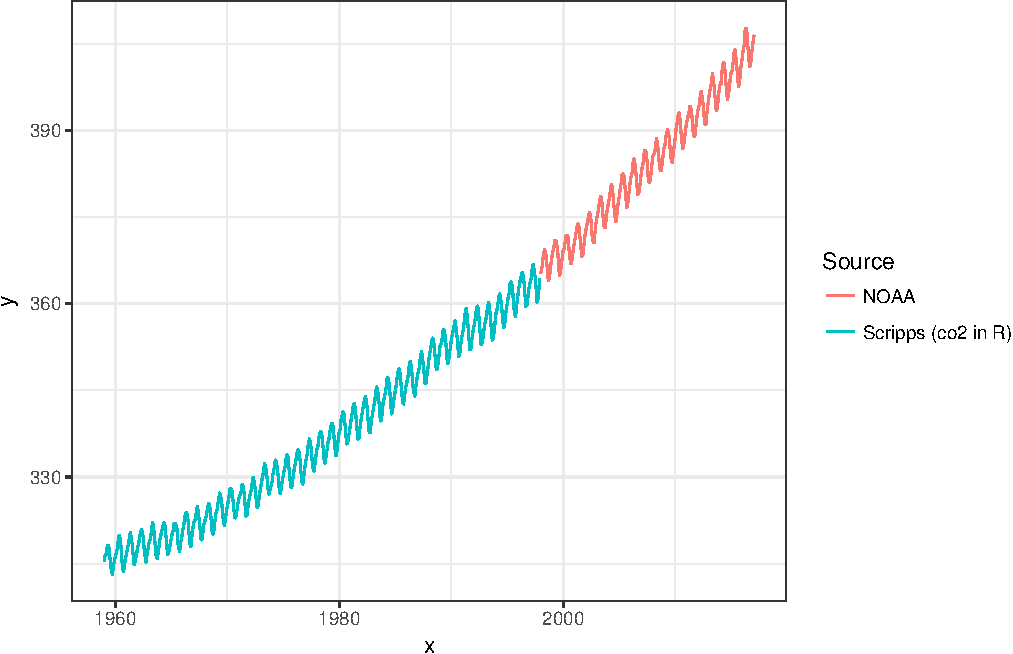
\includegraphics[width=\textwidth]{Lec14_files/figure-beamer/unnamed-chunk-14-1} \end{center}

\end{frame}

\begin{frame}[t]{%
\protect\hypertarget{gp-model}{%
GP Model}}

Based on Rasmussen 5.4.3 (we are using slightly different data and
parameterization)

\[ \symbf{y} \sim \mathcal{N}(\symbf{\mu},~ \symbf{\Sigma}_1 + \symbf{\Sigma}_2 + \symbf{\Sigma}_3 + \symbf{\Sigma}_4 + \sigma^2 \mathit{I}\,) \]

\[\{\symbf{\mu}\}_i = \bar{y}\]

\[
\begin{aligned}
\{\symbf{\Sigma}_1\}_{ij} &= \sigma^2_1 \exp\left(-(l_1 \cdot d_{ij})^2\right) \\
\{\symbf{\Sigma}_2\}_{ij} &= \sigma^2_2 \exp\left(-(l_2 \cdot d_{ij})^2\right)\exp\left(-2 \, (l_3)^2  \sin^2(\pi \, d_{ij} / p)\right) \\
\{\symbf{\Sigma}_3\}_{ij} &= \sigma^2_3 \left(1+\frac{(l_4 \cdot d_{ij})^2}{\alpha}\right)^{-\alpha} \\
\{\symbf{\Sigma}_4\}_{ij} &= \sigma^2_4 \exp\left(-(l_5 \cdot d_{ij})^2\right)
\end{aligned}
\]

\end{frame}

\begin{frame}[fragile]{%
\protect\hypertarget{jags-model}{%
JAGS Model}}

\scriptoutput

\begin{Shaded}
\begin{Highlighting}[]
\NormalTok{ml_model =}\StringTok{ "model\{}
\StringTok{  y ~ dmnorm(mu, inverse(Sigma))}

\StringTok{  for (i in 1:(length(y)-1)) \{}
\StringTok{    for (j in (i+1):length(y)) \{}
\StringTok{      k1[i,j] <- sigma2[1] * exp(- pow(l[1] * d[i,j],2))}
\StringTok{      k2[i,j] <- sigma2[2] * exp(- pow(l[2] * d[i,j],2) - 2 * pow(l[3] * sin(pi*d[i,j] / per), 2))}
\StringTok{      k3[i,j] <- sigma2[3] * pow(1+pow(l[4] * d[i,j],2)/alpha, -alpha)}
\StringTok{      k4[i,j] <- sigma2[4] * exp(- pow(l[5] * d[i,j],2))}
\StringTok{      }
\StringTok{      Sigma[i,j] <- k1[i,j] + k2[i,j] + k3[i,j] + k4[i,j]}
\StringTok{      Sigma[j,i] <- Sigma[i,j]}
\StringTok{    \}}
\StringTok{  \}}

\StringTok{  for (i in 1:length(y)) \{}
\StringTok{    Sigma[i,i] <- sigma2[1] + sigma2[2] + sigma2[3] + sigma2[4] + sigma2[5]}
\StringTok{  \}  }

\StringTok{  for(i in 1:5)\{}
\StringTok{    sigma2[i] ~ dt(0, 2.5, 1) T(0,)}
\StringTok{    l[i] ~ dt(0, 2.5, 1) T(0,)}
\StringTok{  \}}
\StringTok{  alpha ~ dt(0, 2.5, 1) T(0,)}
\StringTok{\}"}
\end{Highlighting}
\end{Shaded}

\end{frame}

\begin{frame}{%
\protect\hypertarget{diagnostics}{%
Diagnostics}}

\begin{center}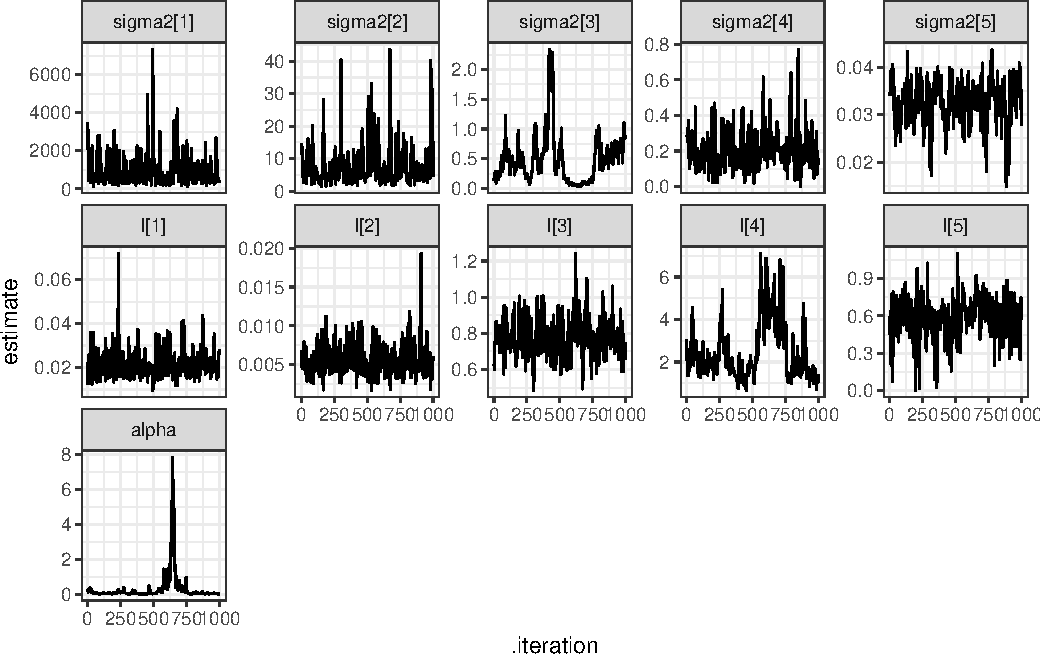
\includegraphics[width=\textwidth]{Lec14_files/figure-beamer/unnamed-chunk-17-1} \end{center}

\end{frame}

\begin{frame}{%
\protect\hypertarget{fit-components}{%
Fit Components}}

\begin{center}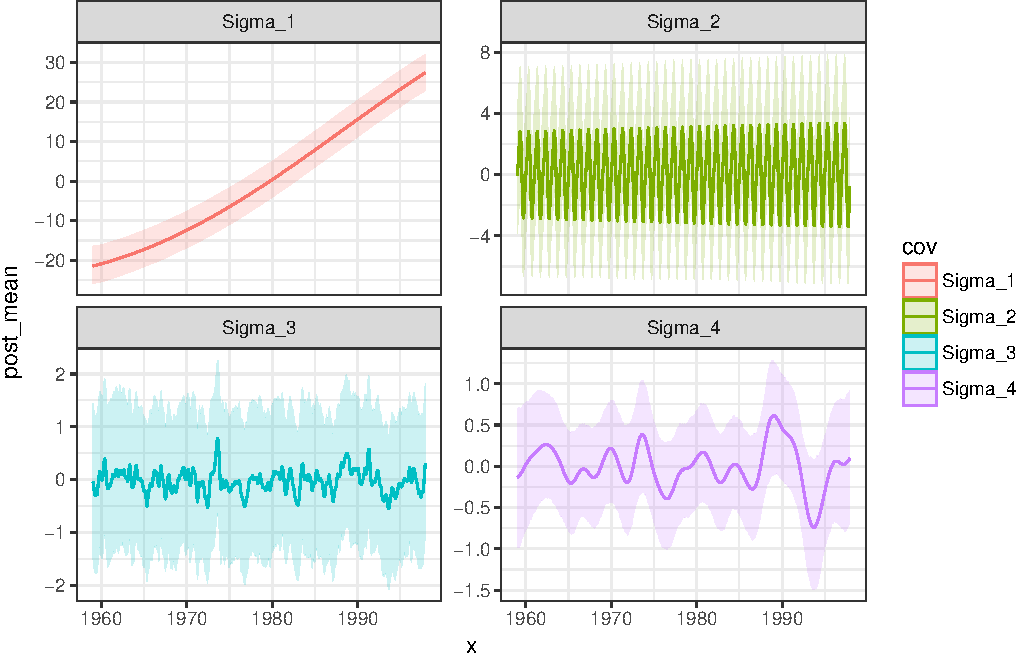
\includegraphics[width=\textwidth]{Lec14_files/figure-beamer/unnamed-chunk-19-1} \end{center}

\end{frame}

\begin{frame}{%
\protect\hypertarget{forecasting}{%
Forecasting}}

\begin{center}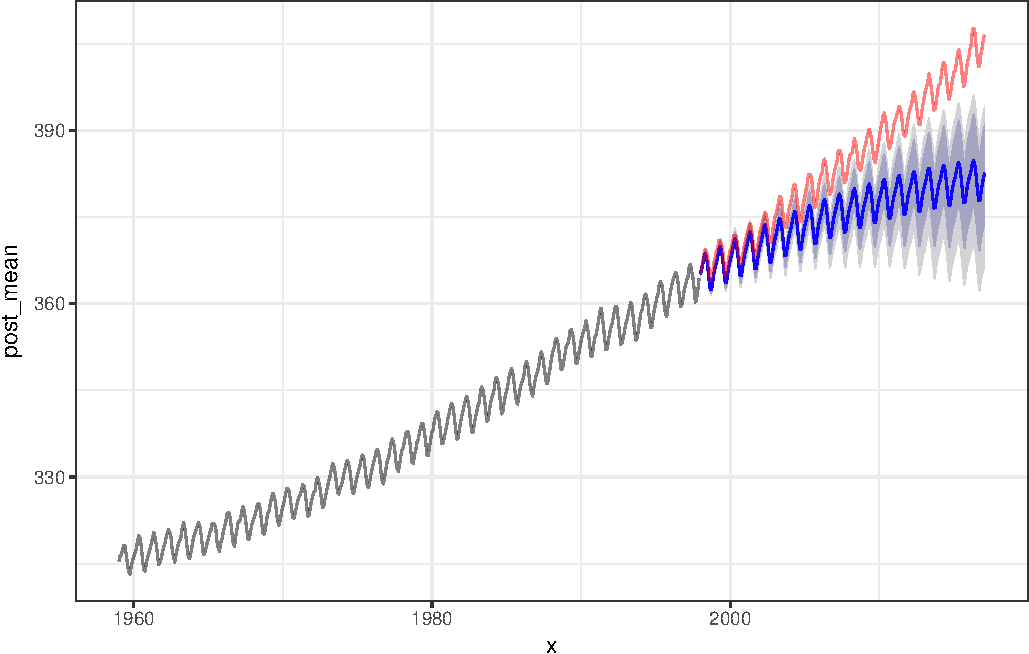
\includegraphics[width=\textwidth]{Lec14_files/figure-beamer/unnamed-chunk-22-1} \end{center}

\end{frame}

\begin{frame}{%
\protect\hypertarget{forecasting-zoom}{%
Forecasting (zoom)}}

\begin{center}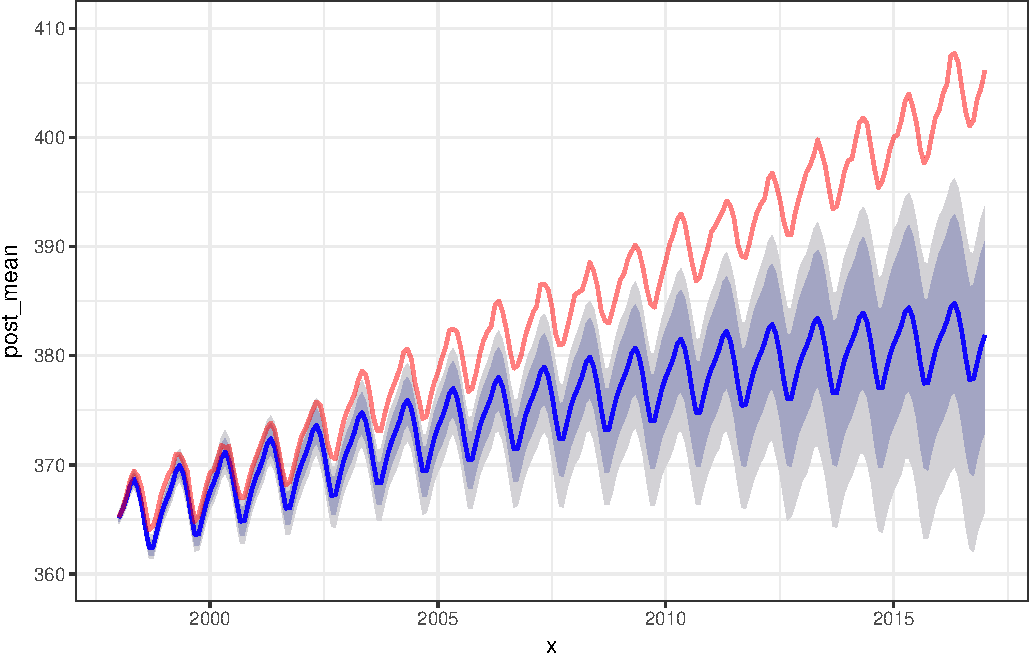
\includegraphics[width=\textwidth]{Lec14_files/figure-beamer/unnamed-chunk-23-1} \end{center}

\end{frame}

\begin{frame}{%
\protect\hypertarget{forecasting-arima-auto}{%
Forecasting ARIMA (auto)}}

\begin{center}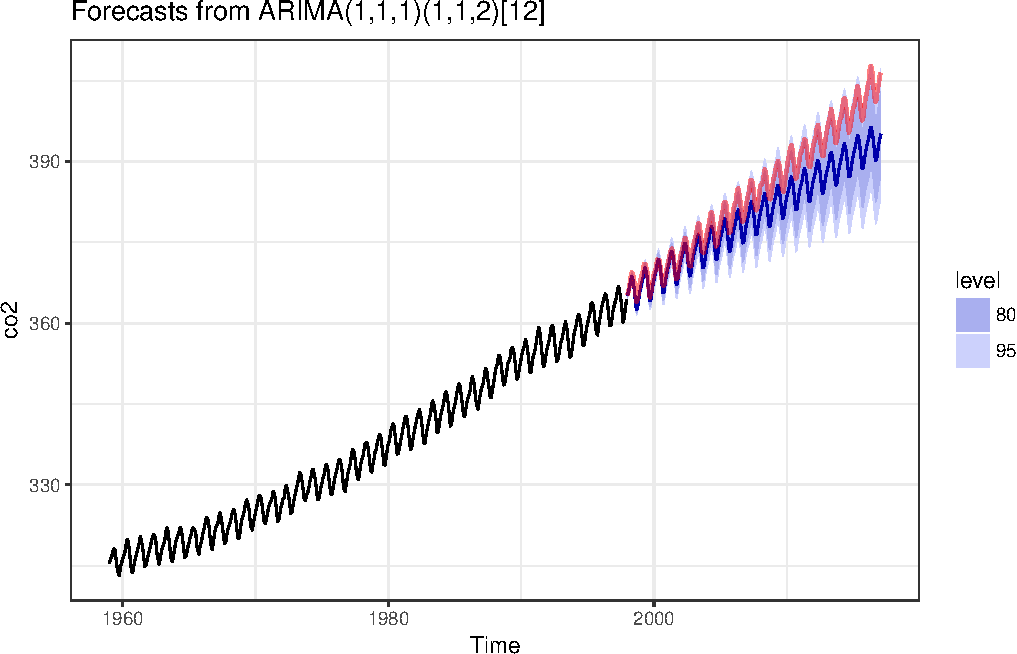
\includegraphics[width=\textwidth]{Lec14_files/figure-beamer/unnamed-chunk-24-1} \end{center}

\end{frame}

\begin{frame}{%
\protect\hypertarget{forecasting-rmse}{%
Forecasting RMSE}}

\begin{longtable}[]{@{}lrr@{}}
\toprule
dates & RMSE (arima) & RMSE (gp)\tabularnewline
\midrule
\endhead
Jan 1998 - Jan 2003 & 1.103 & 1.911\tabularnewline
Jan 1998 - Jan 2008 & 2.506 & 4.575\tabularnewline
Jan 1998 - Jan 2013 & 3.824 & 7.706\tabularnewline
Jan 1998 - Mar 2017 & 5.461 & 11.395\tabularnewline
\bottomrule
\end{longtable}

\end{frame}

\begin{frame}{%
\protect\hypertarget{forecasting-components}{%
Forecasting Components}}

\begin{center}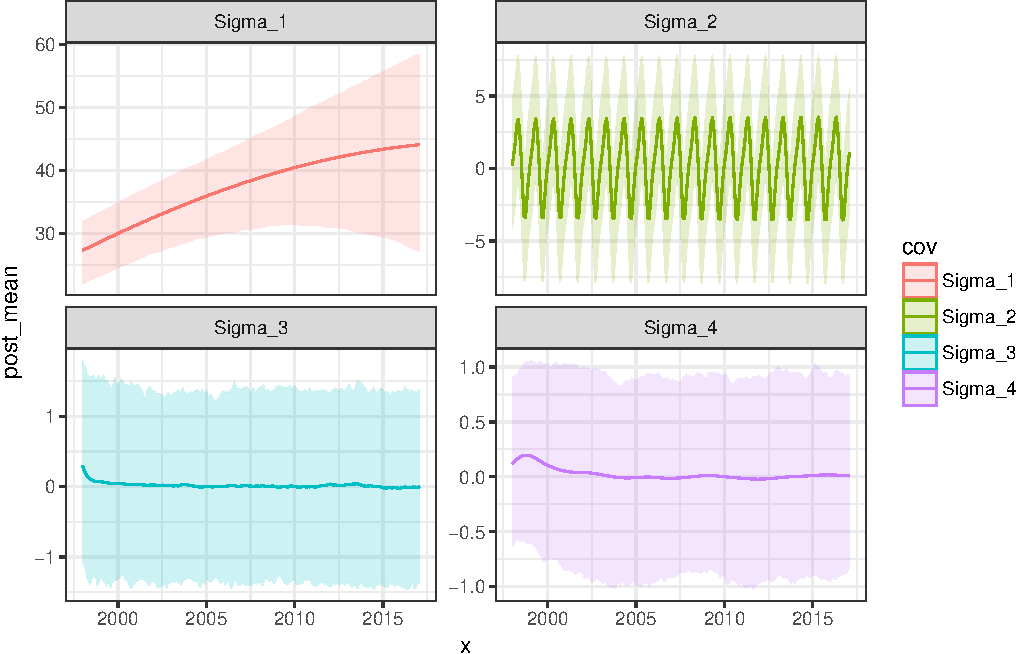
\includegraphics[width=\textwidth]{Lec14_files/figure-beamer/unnamed-chunk-27-1} \end{center}

\end{frame}

\end{document}
